\chapter{Resultados}
\lipsum[1-2]
\begin{comment}


\begin{figure}[!ht]
\begin{subfigure}[b]{.4\textwidth}
  \centering
  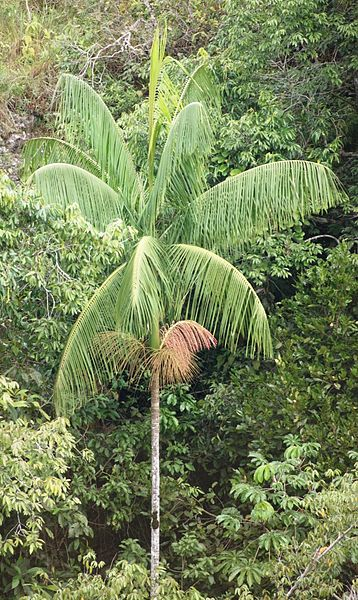
\includegraphics[width=\textwidth]{euteredulis}
  \caption{\textit{Euterpe edulis}}
  \label{fig:eeduli}
\end{subfigure}%
\begin{subfigure}[b]{.4\textwidth}
  \centering
  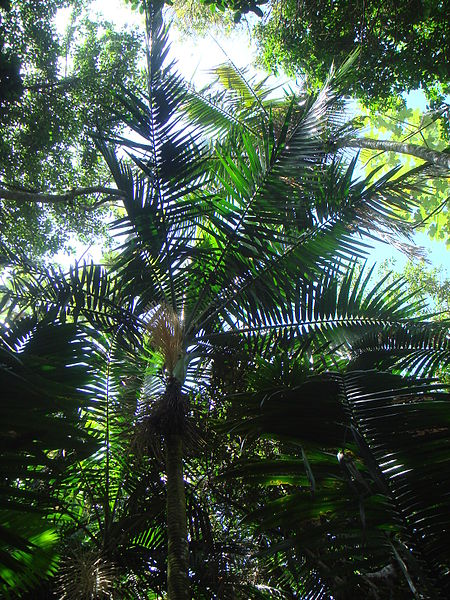
\includegraphics[width=\textwidth]{presacumimon}
  \caption{\textit{Prestoea acuminata}}
  \label{fig:pacumi}
\end{subfigure}
\begin{subfigure}[b]{.4\textwidth}
  \centering
  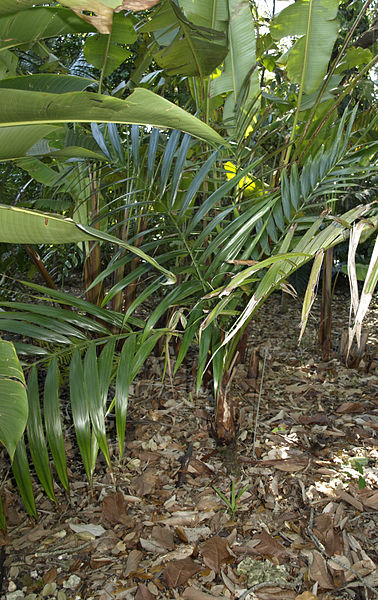
\includegraphics[width=\textwidth]{neoniwatsoni}
  \caption{\textit{Neonicholsonia watsonii}}
  \label{fig:nwatsonii}
\end{subfigure}
\begin{subfigure}[b]{.4\textwidth}
  \centering
  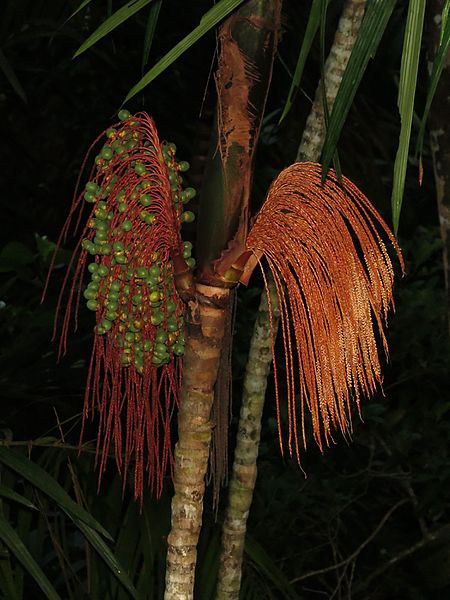
\includegraphics[width=\textwidth]{oenomapora}
  \caption{\textit{Oenocarpus mapora}}
  \label{fig:omapora}
\end{subfigure}
\caption{Genera of palm tribe Euterpeae}
\label{fig:fig}
\end{figure}
\end{comment}

\begin{figure}[!ht]
\centering
\subcaptionbox{\textit{Prestoea acuminata}\label{fig:preacumi}}
{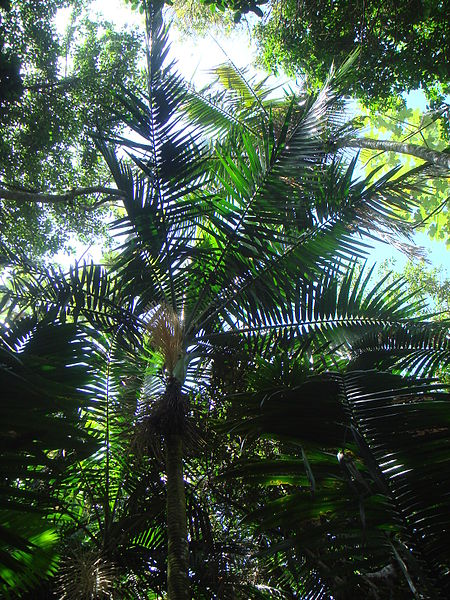
\includegraphics[width=0.4\textwidth]{presacumimon}}
\subcaptionbox{\textit{Oenocarpus mapora}\label{fig:oenomapora}}
{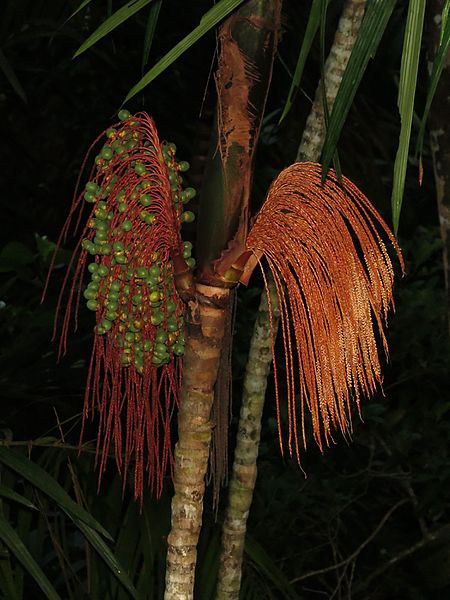
\includegraphics[width=0.4\textwidth]{oenomapora}}
\caption{Ejemplos de taxa dentro de la tribu Euterpeae}\label{animals}
\end{figure}

\lipsum[5-8]

Esto es una referencia a \textit{Prestoea acuminata} (fig.~\ref{fig:preacumi}).
Esto es una referencia a \textit{Euterpe precatoria} (fig.~\ref{fig:euterpreca}).
\begin{figure}[!hb]
\centering
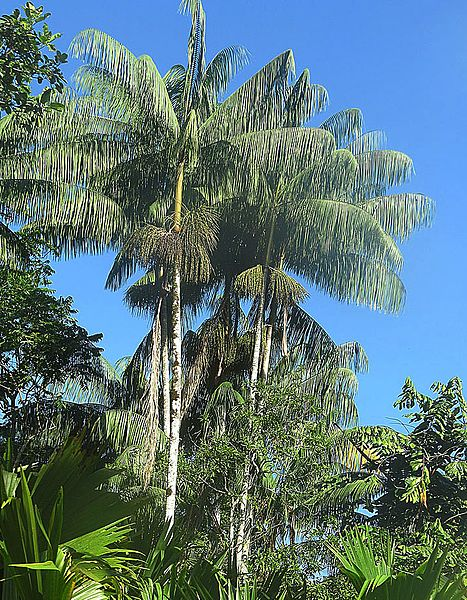
\includegraphics[width=0.5\textwidth]{eprecato}
\caption{Hábito de \textit{Euterpe precatoria}}
\label{fig:euterpreca}
\end{figure}

